% !TeX document-id = {041f4270-ff29-4194-ac21-3def5a3e2038}
% !TeX encoding = UTF-8
% !TeX spellcheck = es_ES
% !TeX root = Tesis.tex
\documentclass[12pt,oneside,openleft]{book}

\usepackage{soul}
\usepackage{easyReview}

\usepackage[letterpaper,lmargin=2.9cm,rmargin=1.9cm,bmargin=2.8cm,tmargin=2.8cm,includeheadfoot]{geometry} % adjusts page layout, showframe

\usepackage{graphicx}  % Add graphics capabilities
\graphicspath{/figures/}
\usepackage{tikz, tikz-3dplot}
\usepackage{flafter}  % Don't place floats before their definition
\usepackage[list=off,font=small,skip=3pt]{caption}
\usepackage{subcaption}

\usepackage{lipsum}
\usepackage{float}

%\usepackage{natbib} % use author/date bibliographic citations
\usepackage{cite}

\usepackage{amsthm}
\usepackage{amsfonts}
\usepackage{amsmath,amssymb}  % Better maths support & more symbols
\usepackage{textcomp} % provide lots of new symbols
\usepackage{bm}  % Define \bm{} to use bold math fonts

\usepackage[utf8]{inputenc} % Any characters can be typed directly from the keyboard
%\usepackage[T1]{fontenc}
\usepackage[spanish]{babel}
\usepackage{color}
\usepackage{xcolor}
\usepackage{colortbl}
\usepackage{longtable}

\usepackage{booktabs}
\setlength{\tabcolsep}{4pt} % General space between cols (6pt standard)
\renewcommand{\arraystretch}{1} % General space between rows (1 standard)

\usepackage{enumitem}
\setlist{itemsep=0.5pt}%nolistsep


\usepackage[plain]{fancyref}
\usepackage[bookmarksopen,colorlinks,pdftex]{hyperref}  % PDF hyperlinks
\hypersetup{citecolor=black,
	        filecolor=black,
	        linkcolor=black,
	        urlcolor=black} % black links, for printed output

\usepackage{fancyhdr}
\fancyhead{\headheight = 14pt}
\fancyhead[LE,RO]{} %\slshape \nouppercase{\rightmark}}
\fancyhead[LO,RE]{\slshape \nouppercase{\leftmark}}
\fancyfoot[C]{\thepage}

\usepackage{aas_macros} %para bibliografía \apj, etc
\usepackage[]{tocbibind} % [nottoc] para remover el indice del toc

%\renewcommand{\baselinestretch}{1.5} % para cambiar interlineado
\usepackage{setspace}
%\usepackage{ieeetran}

\setcounter{secnumdepth}{4} % para numerar subsubsections y parrafos y agregar al toc
\setcounter{tocdepth}{4}
\newcommand{\myparagraph}[1]{\paragraph{#1}\mbox{}\\}

\usepackage{multirow}
\newcommand{\sfref}[1]{{\bfseries figura suplementaria \ref{#1}}}
%\newcommand{\Sfref}[1]{Supplementary figure \ref{#1}}
\newcommand{\stref}[1]{{\bfseries tabla suplementaria \ref{#1}}}
\newcommand{\stsref}[2]{{\bfseries tablas suplementarias \ref{#1} y \ref{#2}}}
\definecolor{tcA}{rgb}{0.811765,0.811765,0.811765}

\makeatletter %eqs en negrita si el texto q lo rodea lo está
\DeclareRobustCommand*{\bfseries}{%
  \not@math@alphabet\bfseries\mathbf
  \fontseries\bfdefault\selectfont
  \boldmath
}
\makeatother

% Para escribir elementos químicos
%\usepackage{chemmacros}
%\usepackage{bohr}
%\newcommand*\mychemistry[2]{%
%  \ch{^{#2}_{\atomicnumber{#1}}#1}}
%\newcommand*\mychemistryg[3]{%
%  \ch{^{#2}_{#3} #1}}
%
%\hyphenation{aproxi-ma-da-men-te}
%\hyphenation{Chandrasekhar}
%\hyphenation{Schwarzschild}

\begin{document}
	
	\selectlanguage{spanish}

    \renewcommand{\tablename}{Tabla}
     \renewcommand{\refname}{Referencias}
    \renewcommand{\figurename}{Figura}

    \renewcommand{\thefootnote}{\Roman{footnote}}

    \lefthyphenmin=2
    \righthyphenmin=2

    \frontmatter

    % !TeX root = Tesis.tex
% !TeX spellcheck = es_ES
% !TeX encoding = UTF-8
\pagestyle{empty}

\newcommand{\HRule}{\rule{\linewidth}{1pt}} % Defines a new command for the horizontal lines, change thickness here

\begin{titlepage}
	
{\begingroup % Create the command for including the title page in the document
	\hbox{ % Horizontal box
%		\hspace*{0.01\textwidth} % Whitespace to the left of the title page
		\rule{1pt}{\textheight} % Vertical line
		\hspace*{0.025\textwidth} % Whitespace between the vertical line and title page text
		\parbox[b][\textheight]{\textwidth}{ % Paragraph box which restricts text to less than the width of the page	
				
\begin{center}			


%\vfill

\Large

Instituto de Cibernética, Matemática y Física 

\smallskip

Departamento de Física Teórica

\vspace{8mm}

%\centerline{\mbox{
%\includegraphics[height=35mm,keepaspectratio]{./logos/logosFF}}}
%\begin{figure}[!h]
%	\begin{subfigure}
%		\includegraphics[height=35mm,keepaspectratio]{./logos/logosFF}
%	\end{subfigure}
%	\begin{subfigure}
%		\includegraphics[height=35mm,keepaspectratio]{./logos/logosUH}
%	\end{subfigure}
%\end{figure}


\begin{minipage}{0pt}
\end{minipage}
\hfill
\begin{minipage}[l]{.18\textwidth}
	\centering
%	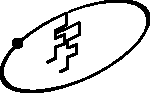
\includegraphics[height=\linewidth,width=\linewidth]{./logos/logoFF}
\end{minipage}
\begin{minipage}[center]{.5\linewidth}
	\centering
	{\Large TESIS DE MAESTRÍA%\\[5pt] \emph{presentada en opción al grado científico de}  \\[5pt] \textbf{Licenciado en Física} % 
	}
\end{minipage}
\begin{minipage}[r]{.18\textwidth}
	\centering
%	
\includegraphics[height=\linewidth,keepaspectratio]{./logos/logoUH}
\end{minipage}\hspace*{10pt}
\hfill
\begin{minipage}{0pt}
\end{minipage}
%\hspace{4pt}


\vfill

% \\[5pt]

\HRule \medskip

%{\LARGE \bfseries \MakeUppercase{Una vista panorámica a los atractores homeostático, Alzheimer y Glioblastoma} %[5pt] %\MakeUppercase{}
%}

{\LARGE \bfseries \MakeUppercase{ Envejecimiento, Alzheimer y Glioblastoma en el espacio de expresión genética} %[5pt] %\MakeUppercase{}
}


\smallskip
\HRule

%%%%%%% FIGURE%%%%%%%%

%%%%%%%%%%%%%%%%%%%%

\vfill

\begin{tabular}{rl}
	
\medskip
\textbf{Autor:} & Joan Andrés Nieves Cuadrado\\
\noalign{\vspace{5pt}}

\textbf{Tutor:}& Dr. Augusto González García,  \textit{ICIMAF}\\ 
			      
\noalign{\vspace{2mm}}
\end{tabular}

\vfill
\begin{minipage}{\linewidth}
	\centering
	
\includegraphics[height=.17\linewidth, keepaspectratio]{./logos/logoICIMAF.png}
\end{minipage}\\[5pt]
\vspace{10pt}
\vfill

\Large
La Habana, 2024


\end{center}

		}}
		\endgroup}

\end{titlepage}
\cleardoublepage

    % !TeX root = Tesis.tex
% !TeX encoding = UTF-8
% !TeX spellcheck = es_ES
\indent
%\section*{Agradecimientos}
%\addcontentsline{toc}{chapter}{Agradecimientos}

\vfill

\begin{quote}
\begin{flushright}
%	\textit{A veces, aceptar ayuda cuesta m\'as que ofrecerla.}\\
%	\textit{Luminara Undulis}
	\textit{Aquí va la dedicatoria o una frase cool}
\end{flushright}



\end{quote}

\vfill
\cleardoublepage

\pagestyle{plain}

	%%\begin{center}
%	\section*{Agradecimientos}
%	%\addcontentsline{toc}{chapter}{Agradecimientos}
%\end{center}
%
%\vfill
%
%\begin{quote}
%	
%Gracias a mi familia, amigos y tutores.
%
%
%
%\end{quote}
%
%\vfill
%\cleardoublepage
%
%\pagestyle{plain}

	% !TeX root = Tesis.tex
% !TeX encoding = UTF-8
% !TeX spellcheck = es_ES
\vfill

\begin{center}
\section*{Resumen}
\addcontentsline{toc}{chapter}{Resumen}
\end{center}
\medskip

\begin{minipage}[c]{.9\linewidth}
\begin{quote}
	
{\large Los datos disponibles de la materia blanca de cerebro permiten localizar los atractores normal (homeostático), Glioblastoma y Alzheimer en el espacio de expresión genética e identificar caminos relacionados con transiciones como la carcinogénesis o la aparición del Alzheimer. También se aprecia una trayectoria predefinida para el envejecimiento, lo cual es consistente con la hipótesis del envejecimiento programado. Adicionalmente, suposiciones razonables sobre la fortaleza relativa de los atractores permite dibujar un panorama esquemático del \textit{fitnest}: diagrama de Wright. Estos sencillos diagramas reproducen relaciones conocidas entre el envejecimiento, el glioblastoma y el Alzheimer, y plantea cuestiones interesantes como la posible conexión entre el envejecimiento programado y el glioblastoma en este tejido. Prevemos que múltiples diagramas similares en otros tejidos podrían ser útiles en el entendimiento de la biología de enfermedades o trastornos aparentemente no relacionados, y para descubrir pistas inesperadas para su tratamiento.}




\end{quote}
\end{minipage}

\smallskip
\vfill
\cleardoublepage

\begin{center}
\section*{Abstract}
\addcontentsline{toc}{chapter}{Abstract}
\end{center}
\medskip

\begin{quote}

{\large Available data for white matter of the brain allows to locate the normal (homeostatic), glioblastoma and Alzheimer’s disease attractors in gene expression space and to identify paths related to transitions like carcinogenesis or Alzheimer’s disease onset. A predefined path for aging is also apparent, which is consistent with the hypothesis of programmatic aging. In addition, reasonable assumptions about the relative strengths of attractors allow to draw a schematic landscape of fitness: a Wright’s diagram. These simple diagrams reproduce known relations between aging, glioblastoma and Alzheimer’s disease, and rise interesting questions like the possible connection between programmatic aging and glioblastoma in this tissue. We anticipate that similar multiple diagrams in other tissues could be useful in the understanding of the biology of apparently unrelated diseases or disorders, and in the discovery of unexpected clues for their treatment.
}


\end{quote}

\vfill
\cleardoublepage

	
    \pagestyle{empty}%fancy

    \singlespacing
    \tableofcontents
	\onehalfspacing
    %\listoffigures
    %\listoftables

    \mainmatter
    \pagestyle{fancy}
    \pagestyle{plain}
    % !TeX root = Tesis.tex
% !TeX encoding = UTF-8
% !TeX spellcheck = es_ES
\chapter*{Introducción} \label{intro}
\addcontentsline{toc}{chapter}{Introducción}
\onehalfspacing

El \textit{fitness} celular refiere a la capacidad de una célula de sobrevivir y proliferar en un ambiente determinado. Abarca varios factores como la capacidad de la célula para adaptarse al ambiente, resistir al estrés y mantener la homeostasis. Este concepto es particularmente importante en la biología del cáncer, donde los niveles de de \textit{fitness} celular pueden determinar su supervivencia y dominancia dentro de un tejido.

Un paradigma conocido en la biología molecular expresa que los máximos locales de \textit{fitness} en el espacio de expresión genética están relacionados con estados biológicos accesibles. Un diagrama de Wright es una representación gráfica reducida del panorama genético, donde los picos y valles representan diferentes genotipos y sus niveles relativos de \textit{fitness} \cite{wright1932roles}, ver figura \ref{fig:wrightDiagram}. 

\begin{figure}[ht]
	\centering
	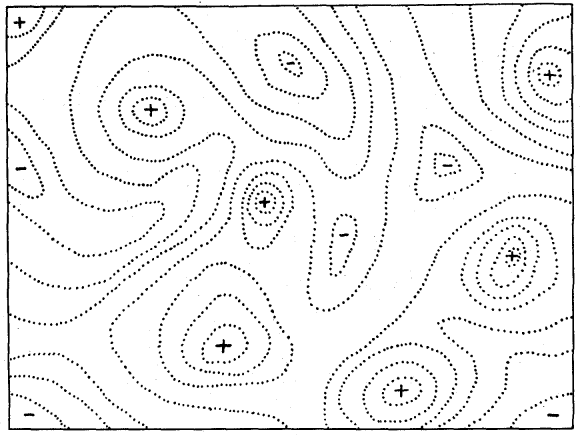
\includegraphics[scale=0.5]{figures/wright_diagram.png}
	\caption{Representación esquemática de un diagrama de Wright. Tomada de la referencia \cite{wright1932roles}}
	\label{fig:wrightDiagram}
\end{figure}

Esta representación ha sido aplicada a la descripción del destino celular a lo largo de una linea de diferenciación \cite{casey2020theory}. Sin embargo, hasta donde sabemos, no hay gráficos basados en datos reales para un tejido dado que represente al menos de forma parcial un diagrama de Wright con más de dos máximos. En el presente trabajo, mostramos un diagrama para la materia blanca del cerebro en el que el estado normal (N) se representa junto con el atractor de glioblastoma (GBM) y el máximo relacionado con la enfermedad del Alzheimer (AD).

La AD se caracteriza por la pérdida progresiva de células neuronales, mientras que el GBM es un tipo de cáncer cerebral que implica la proliferación descontrolada de células. Algunas investigaciones muestran que pacientes con la AD podrían tener un menor riesgo de desarrollar GBM. Por ejemplo, en la referencia \cite{ou2012does} muestran que ambas enfermedades presentan un aumento en el estrés oxidativo, pero en la AD, esto hace que las células neuronales sean más vulnerables a la muerte, mientras que en el GBM, las células cancerosas se vuelven más resistentes. Además, se plantea que la degeneración de células que secretan acetilcolina en la AD podría tener un efecto protector contra el cáncer, ya que esta sustancia puede estimular el crecimiento de células cancerosas.

% Ou
%Claro, aquí tienes un resumen de la relación inversa entre el Alzheimer y el glioblastoma según el artículo que estás viendo:
%
%Enfermedades Contrapuestas: El Alzheimer se caracteriza por la pérdida progresiva de células neuronales, mientras que el glioblastoma es un tipo de cáncer cerebral que implica la proliferación descontrolada de células.
%Estrés Oxidativo: Ambas enfermedades muestran un aumento en el estrés oxidativo, pero en el Alzheimer, esto hace que las células neuronales sean más vulnerables a la muerte, mientras que en el glioblastoma, las células cancerosas se vuelven más resistentes1.
%Acetilcolina: La degeneración de células que secretan acetilcolina en el Alzheimer podría tener un efecto protector contra el cáncer, ya que la acetilcolina puede estimular el crecimiento de células cancerosas.

En \cite{Driver_2012} concluyen que los sobrevivientes de cáncer tienen un riesgo 33 \% menor de desarrollar la AD en comparación con aquellos sin antecedentes de cáncer. Las personas con la AD tienen un riesgo 61 \% menor de desarrollar cáncer.

%Driver
%Claro, aquí tienes un resumen de la relación inversa entre el Alzheimer y el cáncer, según el estudio de Framingham:
%
%Riesgo reducido de Alzheimer en sobrevivientes de cáncer: Los sobrevivientes de cáncer tienen un riesgo 33% menor de desarrollar Alzheimer en comparación con aquellos sin antecedentes de cáncer.
%Menor riesgo de cáncer en pacientes con Alzheimer: Las personas con Alzheimer tienen un riesgo 61% menor de desarrollar cáncer, posiblemente debido a un diagnóstico insuficiente.
%Cánceres relacionados con el tabaco: Los sobrevivientes de cánceres relacionados con el tabaco tienen un riesgo aún menor de Alzheimer, pero un mayor riesgo de accidente cerebrovascular.
%Posibles explicaciones biológicas: La relación inversa podría deberse a mecanismos biológicos compartidos entre el cáncer y las enfermedades neurodegenerativas, como la regulación de la apoptosis y la proteína Pin1.


%roe2009
%Claro, aquí tienes un resumen de la relación entre el Alzheimer y el glioblastoma según el artículo:
%
%Reducción del riesgo: La presencia de Alzheimer (AD) se asocia con un riesgo reducido de hospitalización por cáncer, incluyendo glioblastoma.
%Mecanismos comunes: Se sugiere que mecanismos moleculares comunes podrían estar involucrados en ambas enfermedades, regulando la muerte y supervivencia celular.
%Estudios previos: Otros estudios han mostrado asociaciones similares entre el cáncer y enfermedades neurodegenerativas como el Parkinson.
%Diferencias raciales: La relación entre el cáncer y el Alzheimer varía según la raza, con efectos opuestos observados en minorías, aunque los datos no son concluyentes debido al tamaño de muestra pequeño.


%musicco
%Claro, aquí tienes un resumen del artículo sobre la relación inversa entre el Alzheimer y el cáncer:
%
%Objetivo del estudio: Evaluar la incidencia de cáncer en personas con Alzheimer y la incidencia de Alzheimer en personas con cáncer1.
%Resultados principales: El riesgo de cáncer en pacientes con Alzheimer se redujo a la mitad, y el riesgo de Alzheimer en pacientes con cáncer se redujo en un 35%2.
%Conclusión: Existe una relación inversa entre el Alzheimer y el cáncer, sugiriendo que ambos podrían ser manifestaciones opuestas del envejecimiento.
%
%\alert{El trabajo presentado como tesis de diploma consta de una introducción, tres capítulos,las conclusiones y las recomendaciones. El contenido se distribuye de la siguiente forma:}

\begin{itemize}
	\item[$\bullet$] \textbf{Introducción:}
	
	\item[$\bullet$] \textbf{Capítulo 1:} 
	
	\item[$\bullet$] \textbf{Capítulo 2:} 
	
	\item[$\bullet$] \textbf{Capítulo 3:} 
	
	\item[$\bullet$] \textbf{Conclusiones:} 
	
	\item[$\bullet$] \textbf{Recomendaciones:} 
	
	
\end{itemize}
    % !TeX root = Tesis.tex
% !TeX spellcheck = es
% !TeX encoding = UTF-8
\chapter{Materiales y métodos}
\label{cap1}
\section{Reducción de la dimensionalidad}
\label{c11}
\onehalfspacing

%La reducción de la dimensionalidad es un paso crucial en el análisis de datos, especialmente cuando se trata de grandes conjuntos de datos con muchas variables. Al reducir la dimensionalidad, se facilita la visualización y comprensión de los datos, lo que permite a los analistas y científicos de datos identificar patrones y tendencias importantes. El PCA es una técnica lineal que transforma las variables correlacionadas en un número menor de variables no correlacionadas llamadas componentes principales. Por otro lado, t-SNE y UMAP son técnicas no lineales que son particularmente útiles para preservar la estructura local de los datos en espacios de baja dimensión, lo que las hace ideales para la visualización de agrupaciones complejas y estructuras de datos de alta dimensión. Estas técnicas son herramientas poderosas que ayudan a simplificar la complejidad de los datos sin perder información crítica, lo que permite un análisis más eficiente y efectivo.

La reducción de la dimensionalidad es un paso crucial en el análisis de datos, especialmente cuando se trata de grandes conjuntos con muchas variables. Este facilita la visualización y comprensión de los datos, lo que permite una rápida identificación de patrones y tendencias importantes. Algunas técnicas comunes de reducción dimensional son PCA (\textit{Principal Component Analisis}), t-SNE (\textit{t-Distributed Stochastic Neighbor Embedding}) y UMAP (\textit{Uniform Manifold Approximation and Projection}). Estas técnicas son herramientas poderosas que ayudan a simplificar la complejidad de los datos sin perder información crítica, lo que permite un análisis más eficiente y efectivo.

El t-SNE es un método no linear y estocástico. Su funcionamiento se puede separar en dos etapas. En la primera, se seleccionan los vecinos de cada punto. Para ello se utiliza una distribución gaussiana alrededor de él, donde los más cercanos tienen un probabilidad mayor de ser seleccionados que los lejanos. Este paso permite al modelo preservar las estructuras locales. Durante la segunda etapa, se asignan posiciones iniciales aleatorias en un espacio de menor dimensión (generalmente 2 o 3 dimensiones). Luego, se define una distribución de probabilidad similar para los puntos en el nuevo espacio y se minimiza la divergencia entre las dos distribuciones. Esta etapa ayuda a mantener la fidelidad de la representación en el espacio reducido. De esta forma, el algoritmo logra una transformación de los datos hacia una dimensión reducida que preserva la similitud entre los vecinos cercanos \cite{Maaten2008, Jung_2024}.

UMAP es una técnica muy similar a t-SNE. Una de las diferencias principales es que, durante la selección de los vecinos, se asume que los datos forman una variedad de menor dimensión que el espacio original. Esto le permite ser más eficiente en términos de tiempo de cómputo y más efectivo en la conservación de relaciones a gran escala. Otra característica de este método es que, para hacer la representación reducida, minimiza la entropía cruzada en lugar de la divergencia entre las distribuciones. Estas diferencias permiten a este algoritmo preservar mejor tanto la estructura local como la global de los datos, además de hacerlo capaz de trabajar con datos que no se ajustan necesariamente a una distribución normal. \cite{McInnes2018, Becht_2018}

Por otro lado, el PCA es una técnica lineal y determinista que transforma variables correlacionadas en un conjunto reducido de variables no correlacionadas, conocidas como componentes principales. Al igual que en los casos anteriores, su funcionamiento se puede dividir en dos etapas. En la primera etapa, se centran los datos en su media aritmética y se calcula la matriz de covarianza. Esta matriz captura la variabilidad conjunta entre múltiples variables aleatorias y permite comprender las relaciones entre ellas. Luego, durante la segunda etapa, se obtienen los autovalores, ordenados de mayor a menor, y sus correspondientes autovectores. Los autovectores representan las direcciones de máxima varianza en los datos, mientras que los autovalores indican la cantidad de varianza que se encuentra en cada una de estas direcciones. Al proyectar los datos originales sobre los primeros autovectores, se obtiene una representación de los datos en un sistema ortogonal que maximiza la conservación de la varianza, utilizando el menor número posible de componentes \cite{Lever2017}.

t-SNE y UMAP se han vuelto muy populares últimamente debido a su eficiencia y la gran capacidad de para visualizar datos de alta dimensión en un espacio de 2 o 3 dimensiones. Pero su naturaleza no linear y estocástica hace que sea complejo una interpretación cuantitativa de los resultados. Por otro lado, PCA es una técnica lineal y determinista que junto a su relativa sencillez permite realizar varias interpretaciones de sus resultados.

Sin embargo, la aplicación directa del PCA puede presentar algunas complicaciones. Una de las principales dificultades es la construcción de la matriz de covarianza, ya que el número de elementos que contiene es igual al cuadrado de la dimensión original de los datos. Esto hace que sea imposible almacenarla en la memoria RAM de la mayoría de los equipos de cómputo personales. Por ejemplo, si el número de componentes de los datos es $5 \times 10^4$, la matriz de covarianza tendría $2.5 \times 10^9$ elementos. Suponiendo que cada elemento ocupe 8 bytes, el tamaño total de la matriz sería aproximadamente 19 GB. Si se hace uso de que esta es una matriz simétrica, se podría guardar solo los elementos de la triangular superior (o inferior), permitiendo reducir el almacenamiento necesario casi a la mitad. Sin embargo, aún así se requeriría mucho espacio y este escala rápidamente con el aumento de la dimensión de los datos. Por lo tanto, en general, es necesario recurrir al almacenamiento en disco, que tiene una velocidad de lectura y escritura menor que la memoria RAM.

Otro problema grave que enfrenta el algoritmo estándar del PCA es el cálculo de los autovalores y autovectores. La mayoría de las implementaciones de los métodos directos usados para este cálculo no permiten que se apliquen a grandes matrices debido a las limitaciones de la memoria RAM. Una característica del PCA que resulta de gran ayuda en esta parte es que, en general, no es necesario calcular todos los autovalores, solo los más grandes y sus correspondientes autovectores.

Un algoritmo relativamente sencillo de implementar y que permite calcular solo los autovalores más grandes y  sus correspondientes autovectores es el método de Lanczos. En el caso del análisis de datos de expresión genética, donde solo un subconjunto diferente de genes se expresa en cada tejido, la matriz de covarianza podría tener un número elevado de valores nulos. Esto es beneficioso para el método de Lanczos, ya que funciona mejor con matrices dispersas.

El método de Lanczos puede ser de gran utilidad en algunos problemas donde las implementaciones estándar pueden verse limitadas. Sin embargo, en la práctica se utilizan otras técnicas para realizar el PCA de forma indirecta. Una de las alternativas es la descomposición en valores singulares (SVD, por sus siglas en inglés). %Por estas razones, a continuación mostraremos brevemente la implementación básica del método de Lanczos. Luego, en qué consiste el SVD y cómo realizar el PCA de forma indirecta a partir de este.
A continuación se describirá brevemente como funciona la SVD, algunas de sus propiedades y como realizar el PCA a partir de esta.

%\subsection*{Algoritmo de Lanczos}\label{subsec:lanczos}
%
%El método de Lanczos es una técnica numérica utilizada para encontrar los autovalores y autovectores de una matriz grande y dispersa. Es especialmente útil en problemas de álgebra lineal donde la matriz es demasiado grande para ser manejada por métodos directos.
%
%%TODO
%\alert{Poner aquí el algoritmo general del método de Lanczos}
%
%Una de las limitaciones de este algoritmo es su estabilidad numérica. \alert{Buscar citas} %TODO
%
%\alert{concluir esta idea y enlazar con la siguiente sección}

\subsection*{Descomposición en valores singulares}\label{subsec:svd}

La SVD provee una descomposición numéricamente estable de matrices que puede ser usado en una gran variedad de propósitos. Como resultado de aplicar este algoritmo se obtiene una descomposición matricial única que existe para toda matriz de valores complejos $\mathbf{X} \in \mathbb{C}^{n \times m}$:

\begin{equation}
	\mathbf{X} = \mathbf{U} \mathbf{\Sigma} \mathbf{V}^*,
\end{equation}
donde $\mathbf{U} \in \mathbb{C}^{n \times n}$ y $\mathbf{V} \in \mathbb{C}^{m \times m}$ son matrices unitarias con columnas ortonormales, y $\mathbf{\Sigma} \in \mathbb{R}^{n \times m}$ una matriz con valores reales no negativos en la diagonal y ceros fuera de la diagonal. Aquí $^*$ denota la transpuesta conjugada.

Cuando $n \ge m$, la matriz $\mathbf{\Sigma}$ tiene como máximo $m$ valores distintos de cero en la diagonal y puede ser escrita como $\mathbf{\Sigma} = \begin{bmatrix}\hat{\mathbf{\Sigma}} \\ 0\end{bmatrix}$. Por lo tanto, es posible representar $\mathbf{X}$ de forma exacta usando la versión reducida de SVD:

\begin{equation}
	\mathbf{X} = \mathbf{U} \mathbf{\Sigma} \mathbf{V}^* = \begin{bmatrix} 	\hat{\mathbf{U}} & \mathbf{U}^\perp \end{bmatrix} \begin{bmatrix} \hat{\mathbf{\Sigma}} \\ 0 \end{bmatrix} \mathbf{V}^*,
\end{equation}
las columnas de $\mathbf{U}^\perp$ abarcan un espacio vectorial que es complementario y ortogonal a $\hat{\mathbf{U}}$. Las columnas de $\mathbf{U}$ son llamadas vectores singulares izquierdos de $\mathbf{X}$ y forman una base del espacio de los vectores columnas de $\mathbf{X}$. Las columnas de $\mathbf{V}$ son los vectores singulares derechos y forman una base para los vectores filas de $\mathbf{X}$. Los elementos diagonales de $\hat{\mathbf{\Sigma}} \in \mathbb{C}^{m \times m}$ , los llamados valores singulares, están ordenados de mayor a menor. El rango de $\mathbf{X}$ es igual a la cantidad de valores singulares distintos de cero.

Para ver la relación de esta técnica con el PCA, partimos de la matriz de covarianza. Esta se construye a partir de la siguiente expresión:

\begin{equation}
	\sigma_{ij} = \frac{1}{N - 1}\displaystyle{\sum_{l=1}^{N} \left( x_i^{(l)} - \mu_i \right) \left( x_j^{(l)} - \mu_j \right)},
	\label{eq:covmat1}
\end{equation}

donde $i$ y $j$ son la característica $i$-ésima y $j$-ésima del conjunto de datos estudiado, en nuestro caso son el gen $i$ y $j$, respectivamente. La variable $l$ se recorre por todas las muestras. $\sigma_{ij}$ es el elemento $(i,\ j)$ de la matriz de covarianza, es decir, es la covarianza entre el gen $i$ y el $j$ para los elementos no diagonales y la varianza del gen $i$ para los elementos de la diagonal principal. El número total de muestras es $N$, $x_i^{(l)} \in \mathbb{R}$ es el valor de la componente $i$ en la muestra $l$, y, por último, $\mu_i$ es la media de los valores de la componente $i$ sobre todas las muestras.

Si los datos ya han sido previamente centrados, es decir, se cumple que $\mu_i = 0$ para todo $i$, entonces la ecuación \eqref{eq:covmat1} puede reducirse a:

\begin{equation}
	\sigma_{ij} = \frac{1}{N - 1} \displaystyle{ \sum_{l=1}^{N} x_i^{(l)} x_j^{(l)} },
	\label{eq:covmat2}
\end{equation}

Si definimos una matriz $\mathbf{X} \in \mathbb{R}^{n \times m}$, tal que el elemento $(i,\ j)$ es igual a $x_i^{(j)}/(N-1)$, la ecuación \eqref{eq:covmat2} queda representada en forma matricial como:

\begin{equation}
	\mathbf{C} = \mathbf{X}^T  \mathbf{X}.
\end{equation}

Si usamos la SVD de $\mathbf{X} = \mathbf{U} \mathbf{\Sigma} \mathbf{V}^T$ y la propiedad de ortonormalidad de $\mathbf{U}$ y $\mathbf{V}$, obtenemos:

\begin{eqnarray}
	\mathbf{C} =& \mathbf{V} \mathbf{\Sigma} \mathbf{U}^T \mathbf{U} \mathbf{\Sigma} \mathbf{V}^T, \\
	=& \mathbf{V} \mathbf{\Sigma}^2 \mathbf{V}^T,
\end{eqnarray}
es decir, $\mathbf{\Sigma}$ y $\mathbf{V}$ son la solución del siguiente problema de autovalores:
\begin{equation}
	\mathbf{C} \mathbf{V} = \mathbf{V} \mathbf{\Sigma}^2.
\end{equation}

En otras palabras, cada valor singular de $\mathbf{X}$ distinto de cero es la raíz cuadrada positiva de los autovalores de su matriz de covarianza, y las columnas de $\mathbf{V}$ son los autovectores. En términos del PCA, las columnas de $\mathbf{V}$ son las componentes principales de $\mathbf{X}$ y los elementos de la diagonal de $\mathbf{\Sigma}^2$ representan la varianza de los datos en cada una de las componente.

Esta es la manera usual en la que los algoritmo actuales realizan el PCA, por ejemplo, la librería \emph{scikit-learn} de Python \cite{scikit-learn}. En general, nosotros preferimos usar directamente SVD para hacer el PCA, ya que brinda mayor flexibilidad y control. Por ejemplo, si en lugar usar una matriz de media cero, los datos se centran en el valor medio de un subconjunto, las componentes principales van a indicar la dirección en la cual hay más dispersión respecto a este subjconjunto.

Una ventaja significativa de este método para realizar el PCA, es que se obtiene las componentes principales directamente, sin tener que calcular la matriz de covarianza. Esto permite ahorrar tiempo y recursos computacionales, algo que toma mayor importancia en la medida que aumenta la cantidad de datos y el números de variables a procesar. Un procedimiento similar se siguió en las referencias \cite{Gonzalez_2023, Gonzalez_2021}.

\section{Datos de expresión genética}
Utilizamos datos de expresión genética obtenidos de dos experimentos distintos. El primero de ellos contiene muestras patológicamente normales (o ``sanas'') y con glioma, y fueron tomadas del Atlas del Genoma del Cáncer (TCGA, \href{https://www.cancer.gov/tcga}{https://www.cancer.gov/tcga}) \cite{Brennan_2013, Tomczak2015}. Estas son tomadas durante procedimientos quirúrgicos. Los tumores se pueden localizar en diferente zonas cerebrales pero, como es común en el glioma, estos son tumores tomados de la sustancia blanca del cerebro \cite{ellingson2013probabilistic}.

Hay 5 muestras normales de pacientes con edades en el rango entre 49 y 74 años, mientras que el intervalo de edades de las 169 muestras de glioma es entre 21 y 89 años. Las pacientes femeninas representan aproximadamente dos tercios de la cohorte.

El segundo grupo de datos proviene del estudio longitudinal del Instituto Allen sobre el envejecimiento y la demencia (\href{https://aging.brain-map.org/}{https://aging.brain-map.org/}) \cite{Miller_2017}. Las muestras son tomadas \textit{post mortem}. El grupo de control está conformado por 47 muestras, mientras que en el otro hay 28 muestras. El intervalo de edad para todas estas muestras es entre 77 y 101 años. El diagnóstico de la enfermedad del Alzheimer está respaldado por pruebas cognitivas y otras pruebas clínicas. Alrededor del 40 \% de la cohorte son mujeres.

En ambos experimentos los valores de expresión genética se encuentran en unidades FPKM (\textit{fragments per kilobase of transcript per million fragments mapped}), que es una unidad común en este tipo de estudios. En términos simples, dicha unidad de medida significa: la tasa de fragmentos por base multiplicada por un número muy grande ($ 10^9 $). El cálculo de FPKM para el gen $ i $ se realiza por medio de la siguiente fórmula \cite{Zhao_2021}:

\begin{equation}
	\begin{split}
		FPKM_i &= \frac{q_i}{(l_i/10^3) (\sum_{j}q_j/10^6)} ,\\
		&= \frac{q_i}{l_i \sum_j q_j} * 10^9,
	\end{split}
\end{equation}
donde $ q_i $ es la cantidad de fragmentos contados, $ l_i $ es la longitud del gen, y $ \sum_j q_j $ corresponde al número total de fragmentos.

El uso de esta unidad de medida puede resultar complicado debido a que el valor de expresión genética de muchos genes es cero o muy cercano a cero, mientras que un conjunto muy reducido puede presentar valores entre $10^2$ y $10^4$. Por esta razón, en muchos estudios de análisis de expresión genética se utiliza una variable conocida como expresión diferencial logarítmica ($e_{fold}$). Para un gen determinado $i$, esta se calcula de la siguiente manera:
\begin{equation}
	e^i_{fold} = \log_2\left(\frac{e^i}{e^{i}_{ref}}\right),
\end{equation}
donde $e^i$ es la expresión del gen $i$ y $e^i_{ref}$ es un valor de referencia para dicho gen, ambos en unidades FPKM. Esta nueva variable permite concentrar mejor los puntos, y su distribución tiende a asemejarse a una distribución gaussiana. 

Usualmente, empleamos como valor de referencia del gen $i$ la media geométrica de su expresión en el conjunto de muestras normales (o ``sanas''), tras haber sido desplazadas por una constante pequeña, generalmente $0.1$ o $0.01$. De esta forma, los valores negativos o positivos de la expresión diferencial logarítmica indican la subexpresión o sobreexpresión de un gen, respectivamente.
    % !TeX root = Tesis.tex
% !TeX encoding = UTF-8
% !TeX spellcheck = es_CU-SpanishCuba
\chapter{Diagrama de tres atractores}
\label{cap2}
\onehalfspacing


\section{El diagrama de N + GB + EA}\label{sec:ngbad}

Nuestro punto de partida es el diagrama de los datos de expresión genética del análisis de componentes principales para la materia blanca del cerebro, mostrado en la Fig. \ref{fig:fig1a}. Como se puede notar en la figura, las dos primeras componentes principales capturan más del 80 \% de la varianza del sistema. Por lo tanto, es una representación bidimensional adecuada de la distribución real de los puntos en el espacio de expresión genética.

\begin{figure}[!htb]
	\centering
	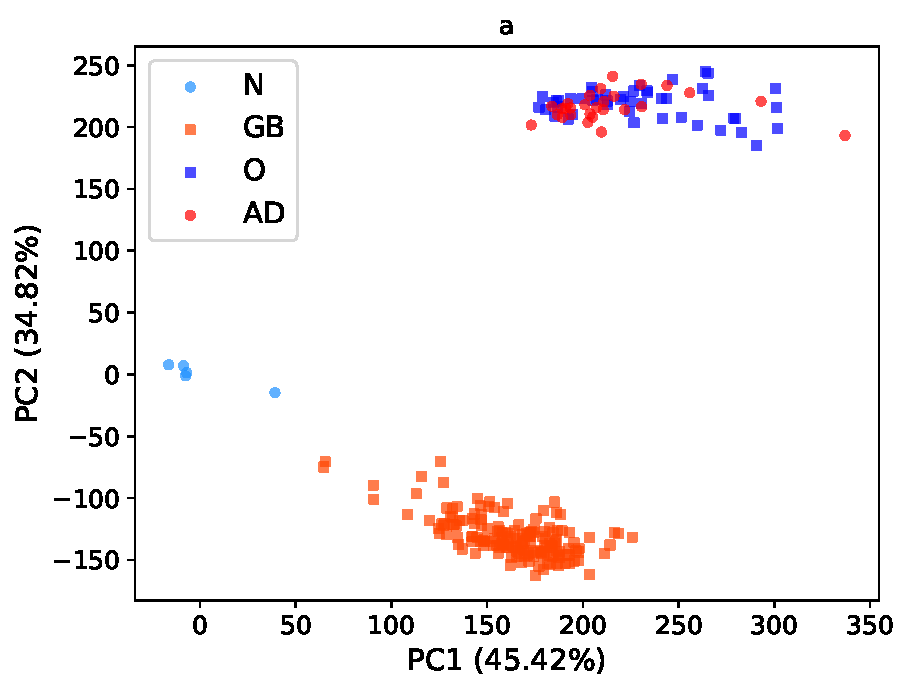
\includegraphics[width=0.75\linewidth]{figures/Fig_1a.pdf}
	\caption{\label{fig:fig1a}
		Análisis de componentes principales para los datos de expresión genética.}
\end{figure}

En la figura se pueden apreciar 4 grupos de muestras. Las muestras marcadas como N y GB corresponden, a especímenes patológicamente normales y tumorales en los datos del TCGA para el glioblastoma \cite{Brennan_2013}. Los centros de las nubes de muestras de N y GB en el espacio de expresión genética definen, respectivamente, los atractores Normal (homeostático) y Glioblastoma de Kauffman \cite{Huang_2009, Gonzalez_2023}. De hecho, la acumulación de puntos en una determinada región de este espacio indica que esta es un atractor de la red de regulación Genética que gobierna la dinámica del sistema.

Por otro lado, los grupos etiquetados como EA y O corresponden a las muestras de la materia blanca del cerebro de la enfermedad del Alzheimer y del grupo de control (\textit{old}) en el estudio del Instituto Allen \cite{Miller_2017}. 

La Fig. \ref{fig:pcaotoad} es una reconstrucción de la figura 3a de la referencia \cite{Gonzalez_2021}. En esta se muestran los resultados del PCA para los datos de expresión genética de la materia blanca del cerebro del Instituto Allen. La primera componente principal (PC1), la cual contiene el $24.7 \%$ de la varianza total, discrimina entre las muestra de O y EA. La posición del centro de la nube de O en este eje es $\left\langle x_1 \right\rangle  = 0 $, y para la EA es $\left\langle x_1 \right\rangle = 40.97 $. Sin embargo, los radios de las nubes de las muestras de O y EA son más grandes que la distancia entre los centros, que son $80.69$ y $72.64$ respectivamente.
%\alert{Estudiamos la transición de O hacia EA en la referencia \cite{Gonzalez_2021}}. En la Fig. \ref{fig:otoad}

\begin{figure}[!htb]
	%TODO:
	\centering
	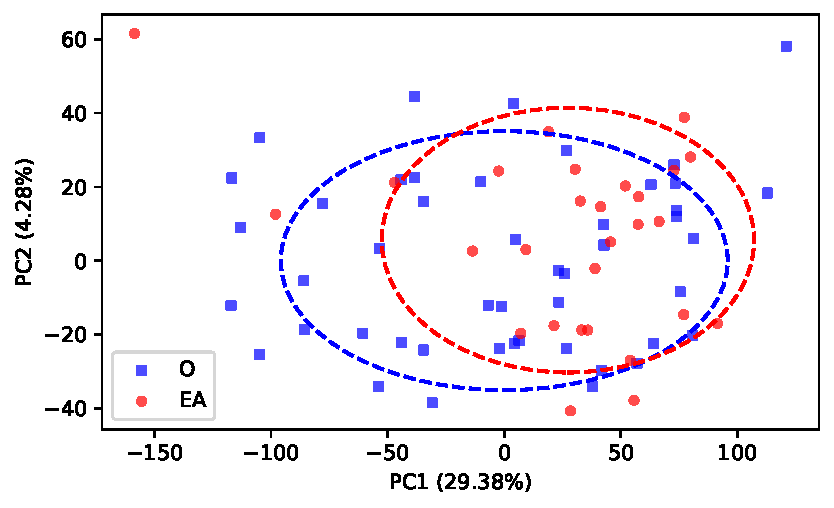
\includegraphics[width=0.75\linewidth]{figures/pca_o_to_ad_1}
	\caption{ Análisis de componentes principales de los datos de expresión genética del Instituto Allen de la materia blanca del cerebro. Se representan las muestras de O y la EA. Las elipses discontinuas se dibujan de acuerdo con las desviaciones estándar de cada conjunto. Tomada de la referencia \cite{Gonzalez_2021}.}
	\label{fig:pcaotoad}
\end{figure}

Es bien conocido el papel de la edad en la EA, especialmente en ancianos \cite{alz2019}. Por lo tanto, podemos usar la edad como una variable de tiempo para seguir la transición. A pesar del número relativamente pequeño de muestras, se realizó un análisis de regresión lineal de la posición media de $\left\langle x_1 \right\rangle$ en función de la edad en las muestras de O, Fig. \ref{fig:otoad}. Esta figura es una reproducción de la 4a de la referencia \cite{Gonzalez_2021} y en la cual se ilustra que $\left\langle x_1 \right\rangle = -287.12 + 3.24 \cdot edad$. En las muestras de la EA, sin embargo, no se encontró correlación entre $\left\langle x_1 \right\rangle$ y la edad observada. Por lo tanto, la posición de la zona EA es aproximadamente fija, y la nube de muestras de O evidencia una deriva hacia el mínimo de la EA a medida que aumenta la edad.

\begin{figure}[!htb]
	\centering
	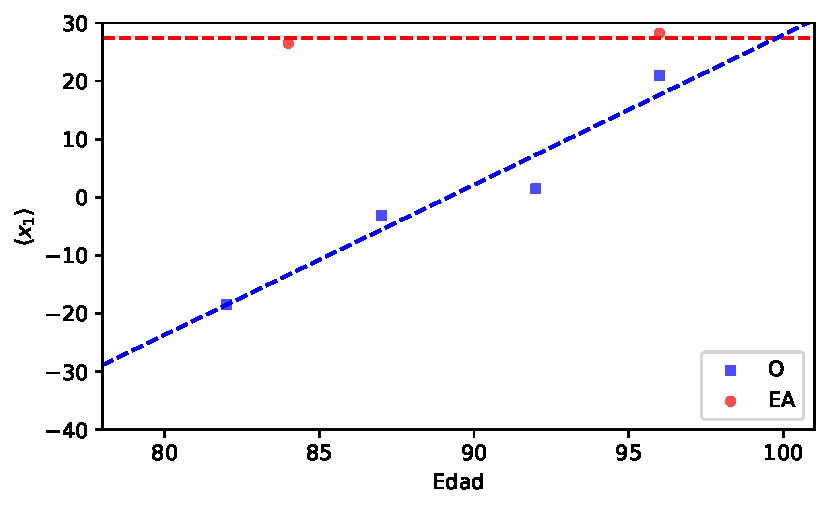
\includegraphics[width=0.75\linewidth]{figures/O_to_AD_1}
	\caption{Posición media de la muestra a lo largo del eje PC1 en función de la edad. A medida que aumenta la edad, las muestras de O experimentan una deriva hacia la región de la EA, cuyo centro es aproximadamente independiente de la edad. Tomada de la referencia \cite{Gonzalez_2021}.}
	\label{fig:otoad}
\end{figure}

Una mejor ilustración de este hecho viene representada en la Fig. \ref{fig:supplotoad}, donde se compara la densidad de probabilidad de las muestras de O y de la EA. Esta reproduce la imagen S2 del material suplementario de la referencia \cite{Gonzalez_2021}. Para construir dicha figura, se definieron cuatro intervalos de edades, que contienen aproximadamente la misma cantidad de muestras de O: [77, 84], [84, 90], [90, 95], [95, 100+]. La probabilidad total de las muestras de la EA es mostrada en los cuatro paneles. El solapamiento creciente entre las densidades de probabilidad evidencia una transición gradual de las muestras del grupo O hacia valores característicos del grupo EA.

\begin{figure}[!htb]
	%TODO: hacer un replot de la figura
	\centering
	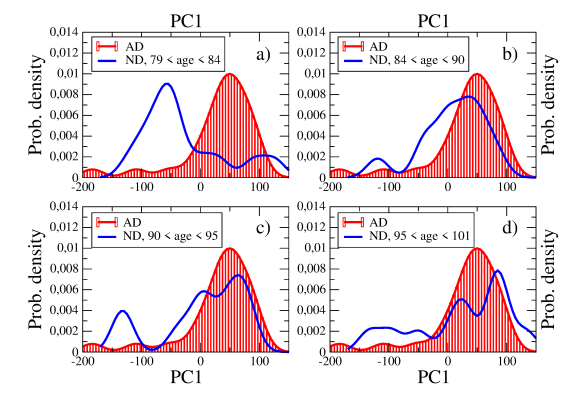
\includegraphics[width=\linewidth]{figures/suppl_otoad}
	\caption{Densidad de probabilidad de las muestras de O y de la EA a lo largo del eje de PC1. Cada panel es para un intervalo de edad para las muestras de O. La probabilidad de la EA, la cual es aproximadamente independiente de la edad, es mostrada en los cuatro paneles. Tomada de la referencia \cite{Gonzalez_2021}.}
	\label{fig:supplotoad}
\end{figure}

Esta propiedad sugiere que el centro de la nube de muestras de la EA define un atractor en el espacio de expresión genética. Las muestras de O parecen ser atrapadas por el atractor de la EA en el proceso del envejecimiento.

Así, en nuestra aproximación, obtenemos un panorama en el espacio de expresión genética de tres atractores: N, GB y EA, y un conjunto de muestras de O que se desplaza hacia la EA. Las posiciones relativas y las principales transiciones entre los atractores se resumen en la Fig. \ref{fig:fig1b}. Asumimos que estas transiciones están determinadas por la biología subyacente a los procesos en los tejidos. La transición de N a la EA se denomina ``EA anticipada'' para enfatizar que también existe una vía hacia la EA a través del envejecimiento: ``EA tardía''. La figura también indica una vía para el GB y para el envejecimiento.

\begin{figure}[!htb]
	\centering
	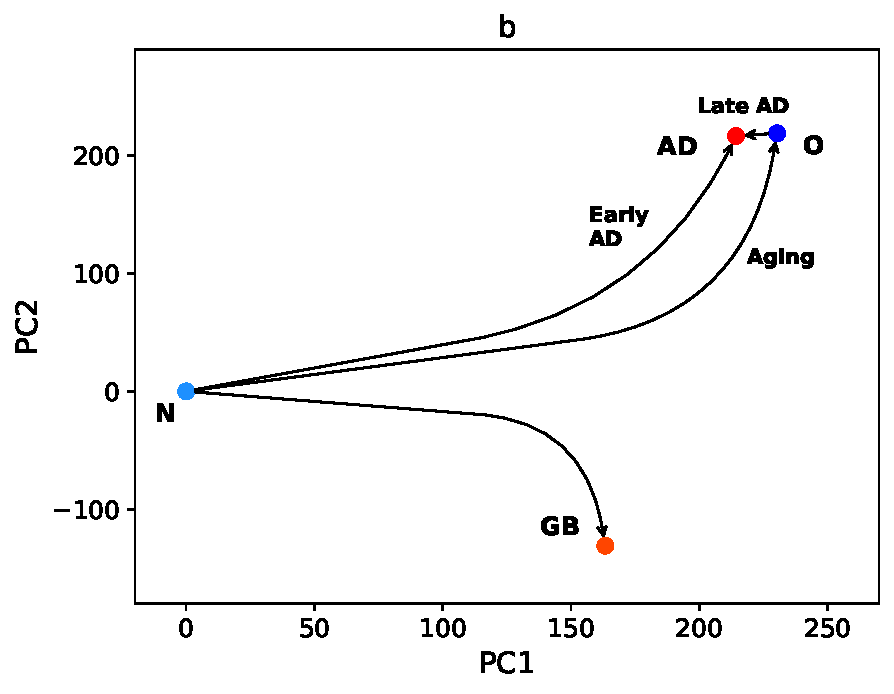
\includegraphics[width=0.75\linewidth]{figures/Fig_1b.pdf}
	\caption{Posiciones relativas y principales transiciones entre los atractores.}
	\label{fig:fig1b}
\end{figure}

\section{Panorama del \textit{fitness}}\label{sec:sec22}

Existe información cualitativa que puede introducirse en nuestra descripción. Esta se relaciona con una variable de \emph{fitness}, de modo que dibujamos una especie de diagrama de Wright \cite{wright1932roles}. En la Fig. \ref{fig:fig1c} se muestra un diagrama esquemático que contiene un gráfico de contorno hipotético del \emph{fitness}. Los atractores N y GB son máximos de \emph{fitness} y deberían estar separados por una barrera de bajo \emph{fitness} \cite{Gonzalez_2021}. El GB debería ser el máximo más alto de los tres actores representados \cite{Gonzalez_2021, gonzalez2022estimating}. Por otro lado, la transición de O a la EA es casi continua, con un número relativamente pequeño de genes expresados diferencialmente \cite{Gonzalez_2021}. Esto significa que existe una barrera muy pequeña, o incluso una ruta sin barrera, que conecta a O y a la EA. Esperamos una barrera de bajo \emph{fitness} que impida las transiciones directas de N a la EA, y un máximo de la EA pequeño, ya que este atractor se encuentra en la región de bajo \emph{fitness}, lejos de N. 

\begin{figure}[!htb]
	\centering
	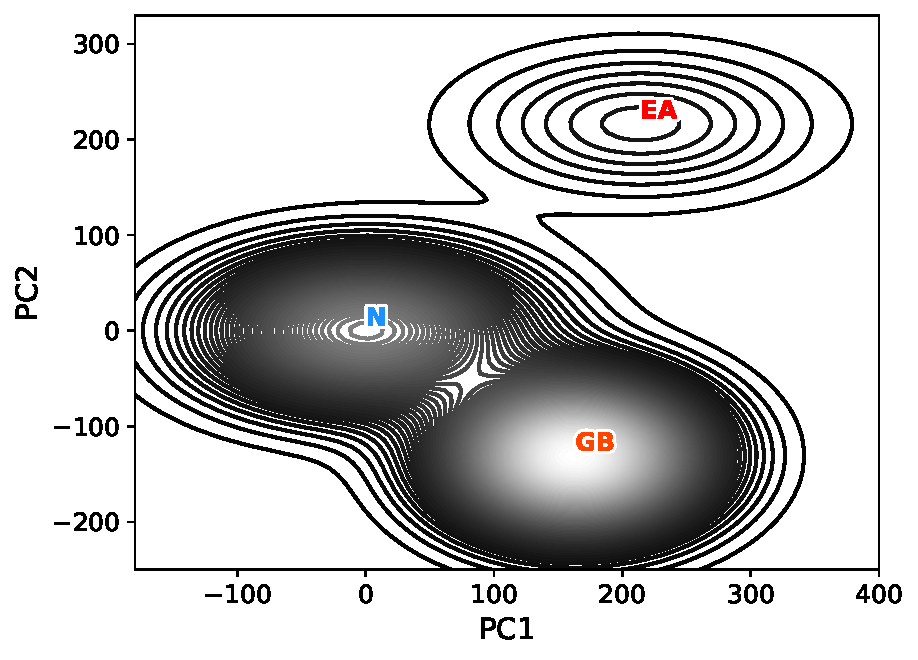
\includegraphics[width=0.75\linewidth]{figures/Fig_1c.pdf}
	\caption{Diagrama de Wright que muestra un gráfico de contorno hipotético del \emph{fitness}. El máximo absoluto corresponde con el estado de GB. El atractor de la EA se representa como un ligero máximo local.}
	\label{fig:fig1c}
\end{figure}

Todos estos hechos se representan en la Fig. \ref{fig:fig1c}. El esquema se construye a partir de una suma de gaussianas centradas en los atractores, con desviaciones estándar proporcionales a los valores reales observados en la Fig. \ref{fig:fig1a} y con alturas que respetan cualitativamente la fuerza relativa de los atractores.

Resaltemos el significado de un diagrama de Wright en el tejido cerebral. En otros tejidos, la evolución somática se relaciona principalmente con la replicación de células madre. Sin embargo, en su estado normal, el cerebro es un tejido de replicación muy lenta \cite{spalding2005retrospective}. Los cambios en pequeñas regiones cerebrales, es decir, los desplazamientos en el diagrama, son básicamente daños acumulados, es decir, envejecimiento \cite{schumacher2021central}. Sin embargo, una vez que se produce la transición al estado GB, se produce un enorme aumento de la tasa de replicación de las células tumorales. Observemos, además, que los cambios relacionados con el envejecimiento son muy evidentes en la sustancia blanca \cite{guttmann1998white}.


\section{Limitaciones}\label{sec:limitations}

En este trabajo se utilizaron datos de expresión genética, en formato FPKM, de las referencias \cite{Brennan_2013, Miller_2017}. Estos fueron obtenidos usando diferentes plataformas. Nosotros tomamos aproximadamente 30 000 genes que están perfectamente identificados en ambas plataformas y realizamos un sencillo análisis de componentes principales \cite{Lever2017}, como se definió en la sección \ref{subsec:svd}. Para definir los valores de la expresión diferencial logarítmica y calcular la matriz de covarianza utilizada para el PCA, se utilizó como referencia común la media geométrica en el conjunto de muestras N.

Debido al uso de estos datos, proveniente de dos experimentos distintos, para realizar un solo calculo de PCA surgen problemas tanto técnicos como conceptuales. Por ejemplo, la referencia N corresponde precisamente al estado normal del cerebro, sino que son un conjunto de muestras patológicamente normales que fueron tomadas de individuos con GB. Además, dos de los pacientes tienen más de 70 años. Desde el punto de vista computacional, por otro lado, se podrían utilizar correcciones por lotes\cite{haghverdi2018batch, zhang2020combat}, que corrigen parcialmente los sesgos asociados a cada grupo de muestras, pero también pueden introducir problemas incontrolados.

En lugar de introducir procedimientos muy avanzados, preferimos extraer los datos directamente de las fuentes y utilizar la técnica de PCA más sencilla. No creemos que ninguna corrección altere sustancialmente el análisis cualitativo derivado del diagrama de tres atractores que se muestras en la Fig. \ref{fig:fig1a}.

La situación ideal podría ser repetir el experimento dentro de un único marco tecnológico, incluyendo datos de personas jóvenes sanas, que se utilizarían para establecer la referencia de los cálculos de la expresión genética diferencial, incluyendo datos de pacientes con GB y la EA, y datos de pacientes sanos en diferentes rangos de edad. Este es un experimento complejo, pero podría ser particularmente factible en un modelo de ratones \cite{hahn2023atlas}, por ejemplo. Consideramos nuestro diagrama de la Fig. \ref{fig:fig1a} como una aproximación cualitativa de este experimento ideal.
    % !TeX root = Tesis.tex
% !TeX encoding = UTF-8
% !TeX spellcheck = es_CU-SpanishCuba
\chapter{Resultados}
\label{cap3}
\onehalfspacing

\section{Principales resultados}

Sobre la base de nuestros diagramas, podemos formular las siguientes observaciones o afirmaciones, que son los principales resultados del trabajo.

\begin{enumerate}
	\item  \textbf{Existe una dirección en el espacio de expresión genética, que a grandes rasgos se puede identificar con el eje PC1, asociada al envejecimiento y a un aumento del riesgo de padecer GB y la EA.}
\end{enumerate}

De hecho, el desplazamiento en esta dirección implica escalar parcialmente las barreras de bajo \textit{fitness} que separa N de los estados GB y EA, y por lo tanto aumentar el riesgo tanto para GB como para la EA.

Vale la pena observar los principales genes involucrados en este proceso. Para ello, observamos el vector unitario a lo largo del eje PC1. Los genes se clasifican según su contribución al vector unitario.% \alert{El procedimiento es similar al algoritmo de Page Rank \cite{Duhan_2009}. Lo usamos en nuestro trabajo anterior \cite{Gonzalez_2023}.}

En la Tabla \ref{tab:apx3} de los apéndices se encuentra una lista con los 100 primeros genes del \textit{ranking}. En la Fig. \ref{fig:figpc1} se representan los valores de los 30 primeros genes en el vector PC1 ordenados por su valor absoluto. Las amplitudes positivas definen genes cuya expresión aumenta con el desplazamiento a lo largo de la dirección positiva de PC1, mientras que las amplitudes negativas se refieren a genes silenciados. Estos genes deberían desempeñar simultáneamente un papel crucial en el envejecimiento, el GB y la EA.

\begin{figure}[!htb]
	\centering
	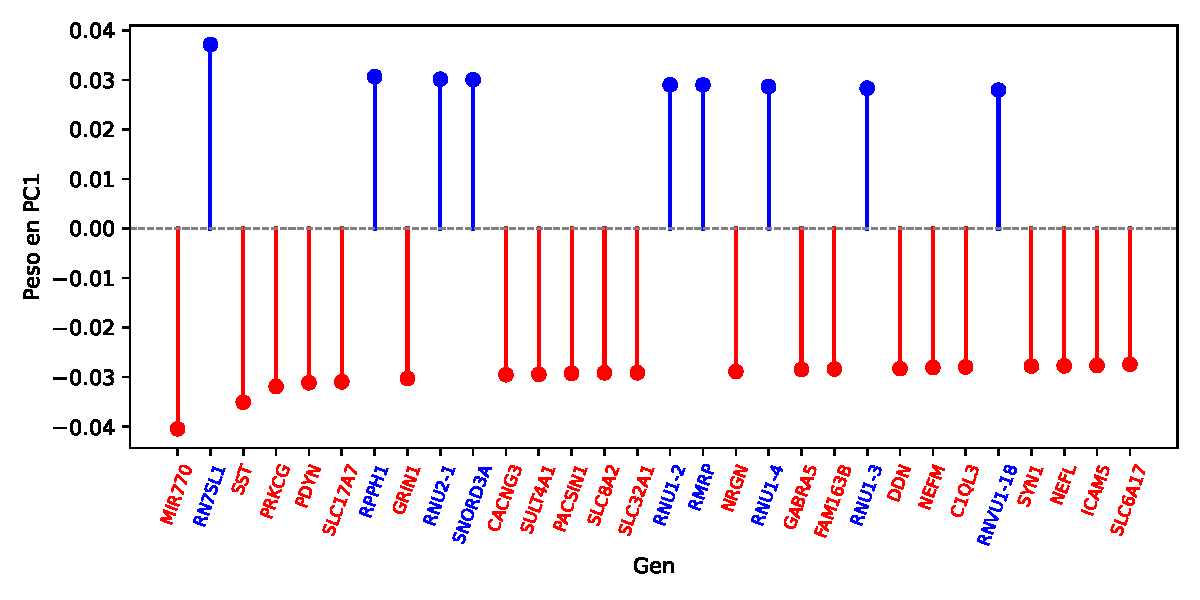
\includegraphics[width=\linewidth]{figures/PC1}
	\caption{Genes con mayor peso a lo largo del vector PC1.}
	\label{fig:figpc1}
\end{figure}

Por supuesto, debido al valor puramente cualitativo de nuestro análisis, los genes, y especialmente el \textit{ranking}, deben considerarse con cautela. Sin embargo, cabe destacar que 20 de los genes silenciados están relacionados con los procesos principales de transmisión a través de sinapsis químicas. En la Tabla \ref{tab:apx4} del Apéndice \ref{apx:apx3} se enumeran los procesos principales del \textit{Reactome} (\href{https://reactome.org/}{https://reactome.org/}) asociadas a estos genes \cite{Gillespie_2021}. Este conjunto incluye 56 genes anotados.

La disminución de la función sináptica es una característica conocida del cerebro envejecido, según la revisión \cite{Ham_2020}. La segunda característica principal, según esta referencia, es un aumento de la función inmunitaria, que no es particularmente evidente en nuestro conjunto de genes. En cambio, observamos genes relacionados con la neurotoxicidad de las toxinas de clostridium \cite{Biazzo_2022}, con la disminución de la actividad mitocondrial \cite{Sun_2016}, micro ARN compartidos entre la EA y el GB \cite{Thomas_2020}, etc.

\begin{enumerate}
	\item[2.] \textbf{Hay una dirección en el espacio de expresión genética, que puede identificarse aproximadamente con el eje PC2, que muestra que la EA y GB son alternativas excluyentes.}
\end{enumerate}

De hecho, la EA y el GB aparecen en semiplanos opuestos. La evidencia clínica \cite{ou2012does, Driver_2012, Roe_2010, Musicco_2013} y los estudios de biología molecular \cite{Liu_2013, Lanni_2020} respaldan esta disyunción. En consecuencia, el eje PC2 involucra genes con desregulación inversa en la EA y el GB.

En la Tabla \ref{tab:apx5} de los apéndices, se listan los 100 genes principales definidos por el vector unitario a lo largo del eje PC2. En la Fig. \ref{fig:figpc2} se representa gráficamente la contribución a dicho vector de los 30 primeros genes ordenados por su valor absoluto. Los pesos positivos corresponden a genes cuya expresión aumenta en la transición de N a la EA. Por otro lado, las amplitudes negativas corresponden a genes cuya expresión aumenta en la transición de N a GB.

\begin{figure}[!htb]
	\centering
	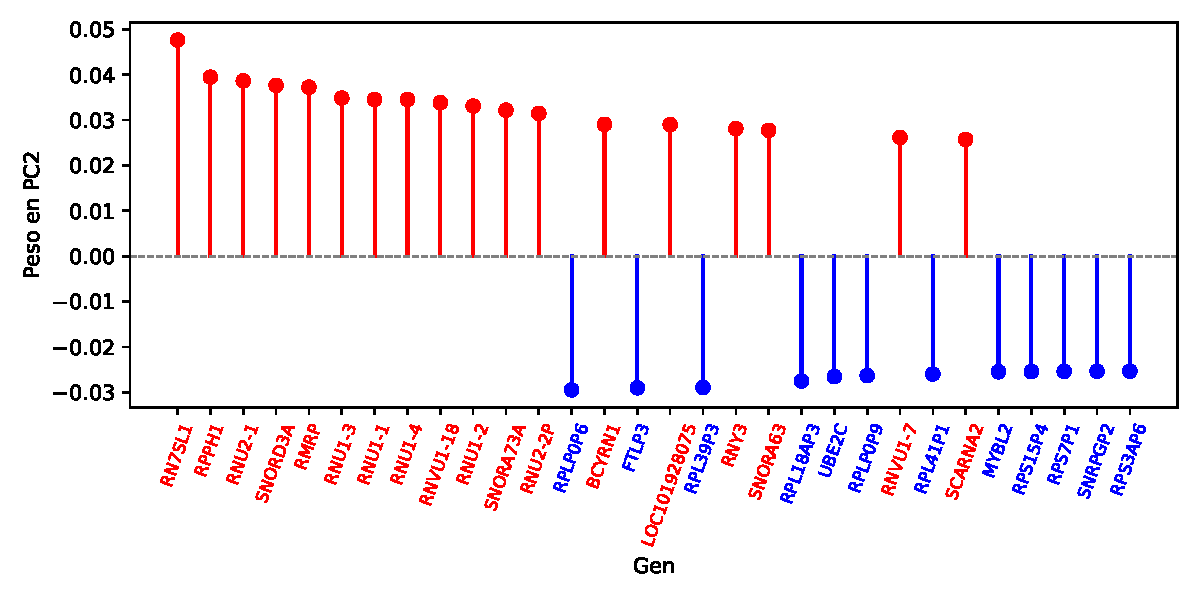
\includegraphics[width=\linewidth]{figures/PC2}
	\caption{Genes con mayor peso a lo largo del vector PC2.}
	\label{fig:figpc2}
\end{figure}

Los procesos de \textit{Reactome} relacionadas con estos genes se muestran en la Tabla \ref{tab:apx6} del Apéndice \ref{apx:apx5}. Se relacionan principalmente con el control del ciclo celular, la replicación del ADN, la apoptosis, la modificación de la matriz extracelular, etc., es decir, con las características distintivas del cáncer \cite{Hanahan_2000, Hanahan_2011, Hanahan_2022}.

Anteriormente, mencionamos MMP9 como un ejemplo de genes que desempeñan funciones opuestas en el GB y la EA. El gen codificador de la proteína UBE2C es otro gen conocido con esta característica \cite{MA_2016, Jaladanki_2021}. Por otro lado, el gen BCYRN1, también entre los primeros 100 genes del \textit{ranking}, parece estar subexpresado en GB \cite{Mu2021} y sobreexpresado en la EA \cite{Zhang_2021}. La Fig. \ref{fig:fig1d} muestra gráficos de violín para la expresión diferencial de los genes MMP9 y BCYRN1 en muestras de N, GB y la EA.

\begin{figure}[!htb]
	\centering
	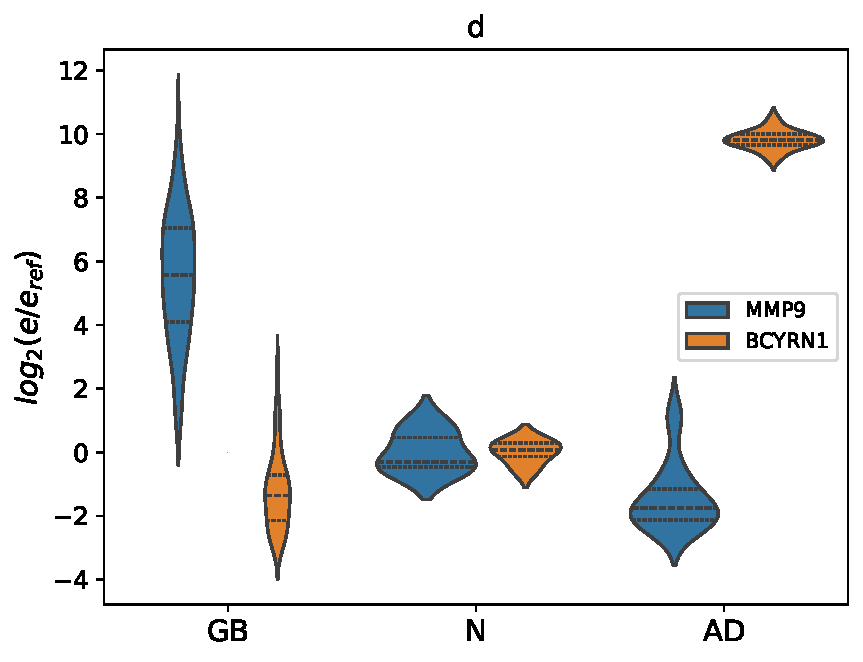
\includegraphics[width=0.75\linewidth]{figures/Fig_1d.pdf}
	\caption{Gráficos de violín para la expresión diferencial logarítmica de los genes MMP9 y BCYRN1 en los estados N, GB y EA.}
	\label{fig:fig1d}
\end{figure}

Noté también que en la Tabla \ref{tab:apx5} hay numerosos genes codificadores de proteínas ribosomales, de núcleo pequeño, de microARN y de otros tipos, regulados inversamente en ambos procesos. Solo 18 de este conjunto de genes están anotados en los procesos \textit{Reactome}. Este es un problema habitual en el análisis de procesos, donde las funciones biológicas de muchos genes no están anotadas.

\begin{enumerate}
	\item[3.] \textbf{Existe un corredor de envejecimiento, es decir un camino preferencial para el envejecimiento en el espacio de expresión genética.}
\end{enumerate}

En nuestros datos, existen muestras en la región N y muestras correspondientes a cerebros de edad normal, ubicadas en una región definida cerca del atractor de la EA. En otras palabras, el proceso de envejecimiento parece definir una trayectoria o corredor de decrecimiento continuo del \textit{fitness}, del cual los datos O muestran el último segmento. Sin embargo, faltan muestras en la región intermedia.

En lugar de incluir muestras adicionales en nuestra figura, lo cual introduciría efectos de lote adicionales, utilizamos resultados recientes en un modelo de ratón \cite{hahn2023atlas} que muestran indudablemente un corredor continuo para el envejecimiento. Presentamos en la Fig. \ref{fig:suppl1} del Apéndice \ref{apx:apx1} una representación gráfica de sus datos para el cuerpo calloso, una región rica en materia blanca. En el panel izquierdo, se grafican las dos primeras componentes principales para los centros de los subgrupos de muestras. Se consideran edades de ratón entre 3 y 28 meses; este último equivale aproximadamente a 80 años en una escala humana. Un corredor para el envejecimiento es evidente. El panel derecho, por otro lado, muestra distancias reales incluyendo todos los componentes. Por lo tanto, las proyecciones en el plano (PC1, PC2) son una representación fiel de la distribución real de puntos.

En nuestro esquema (Fig. \ref{fig:fig1b}), se delinea un corredor de envejecimiento. La Fig. \ref{fig:fig1c} sugiere que este corredor es una dirección con una mínima disminución del \textit{fitness}.

Una dirección o corredor preferencial para el envejecimiento es consistente con la hipótesis del envejecimiento programado \cite{Magalh_es_2012, Gems_2022}, es decir, la idea de que el envejecimiento está programado en nuestros genes.

\begin{enumerate}
	\item[4.] \textbf{El corredor de envejecimiento predeterminado podría estar relacionado con la presión de evitar el fuerte atractor GB.}
\end{enumerate}

Una pregunta muy interesante se refiere a la selección de la dirección preferida para el envejecimiento. Nuestro esquema simplificado (Fig. \ref{fig:fig1c}) ofrece una respuesta inesperada: en la materia blanca, esta dirección podría estar relacionada con la presión para evitar el atractor GB más fuerte.

De hecho, para cada pequeña porción de tejido, se puede modelar el envejecimiento como una especie de movimiento aleatorio que comienza en la región N. Obsérvese que en la referencia \cite{Herrero_2022} se utilizó un modelo de saltos aleatorios en el espacio de expresión genética para describir la evolución somática de diferentes tejidos hacia el cáncer. Primero, asumimos que la dirección de los saltos es aleatoria en el plano que se muestra en la Fig. \ref{fig:fig1c}.

Solo existen cuatro posibilidades para el destino de las trayectorias aleatorias en el plano que comienzan en la región N. Primero, la trayectoria permanece en la región N. Segundo, llega a una región de \textit{fitness} muy baja y las células mueren. Este es el destino de muchas células en el cerebro envejecido. Tercero, es capturada por el atractor GB. Y, finalmente, la cuarta posibilidad es la captura por el atractor de la EA.

Debido al elevado valor de \textit{fitness} del atractor GB, debería existir una probabilidad relativamente alta de que las trayectorias sean capturadas por el GB, lo que conduce a la iniciación de un tumor. Esto implica un enorme aumento del \textit{fitness}, la propagación del tumor en el cerebro y una esperanza de vida para el individuo de tan solo unos dos años tras la iniciación \cite{Poon_2020}. Esto podría afectar a los individuos en edad reproductiva. Por lo tanto, evitar el atractor GB podría ser objeto de la presión selectiva.

Como comprobación indirecta, podemos comparar las incidencias de GB y la EA. Estas deberían ser proporcionales a las tasas de captura de trayectorias aleatorias por los atractores de GB y EA. Como se mencionó, en un modelo donde la dirección de los saltos es aleatoria, la incidencia de GB debería ser mucho mayor que la de la EA. Sin embargo, la incidencia global del glioblastoma es inferior a 10 por 100 000 personas \cite{Ohgaki2005}, en contraste con el 5 \% de la EA en personas de 65 a 74 años y el 13 \% en personas de 75 a 84 años \cite{alz2023}. La incidencia observada sugiere que se evita el movimiento hacia el centro de GB.

\begin{enumerate}
	\item[5.] \textbf{La aparición tardía de la EA podría ser el resultado de la captura por parte del atractor de la EA de microestados cerebrales envejecidos.}
\end{enumerate}

La imagen es, por lo tanto, la siguiente. El proceso de envejecimiento se relaciona inicialmente con un desplazamiento a lo largo del corredor de envejecimiento, con la correspondiente disminución del \textit{fitness}. En los últimos pasos, los estados O son capturados por el atractor débil de la EA.

Como se mencionó anteriormente, la afirmación sobre el corredor de envejecimiento está respaldada por el experimento en un modelo de ratón, mientras que la captura por parte del centro de la EA está sugerida por los cálculos de la referencia \cite{Gonzalez_2021}, particularmente por los resultados que se muestran en la Fig. \ref{fig:otoad}, que es un reconstrucción de la Fig. 4 de esa referencia.

En la Tabla \ref{tab:apx7} se muestran los 10 genes principales en la transición de O a la EA. Se trata de genes incluidos en la Tabla \ref{tab:apx3}, pero que varían en dirección opuesta, es decir, en la dirección negativa del eje PC1. Este hecho se representa en el diagrama esquemático de la Fig. \ref{fig:fig1b}.


\section{Perspectiva cuantitativa}

Debido al carácter cualitativo de nuestro estudio, el análisis de genes y procesos relevantes no se aborda adecuadamente en este artículo. Sin embargo, analicemos cualitativamente siete marcadores conocidos para la EA y el GB según nuestro esquema. Los gráficos de violín para estos genes se muestran en Fig. \ref{fig:violin}. La figura muestra que los genes MAPT (proteína tau \cite{Strang_2019}) y APP (beta amiloide \cite{TCW_2016}) están subexpresados tanto en el GB como en la EA y, por lo tanto, según nuestro esquema, son genes tipo PC1, principalmente relacionados con el envejecimiento. En cierto modo, esto concuerda con los hallazgos del estudio del Instituto Allen sobre los patrones de proteína tau y placas amiloides en el cerebro envejecido. Por supuesto, ciertas mutaciones de estos genes podrían conducir a un envejecimiento cerebral acelerado y a la aparición temprana de la EA. El gen APOE \cite{Raulin_2022}, por el contrario, está desregulado inversamente en el GB y la EA. Es un gen del tipo PC2.

\begin{figure}[!htb]
	\centering
	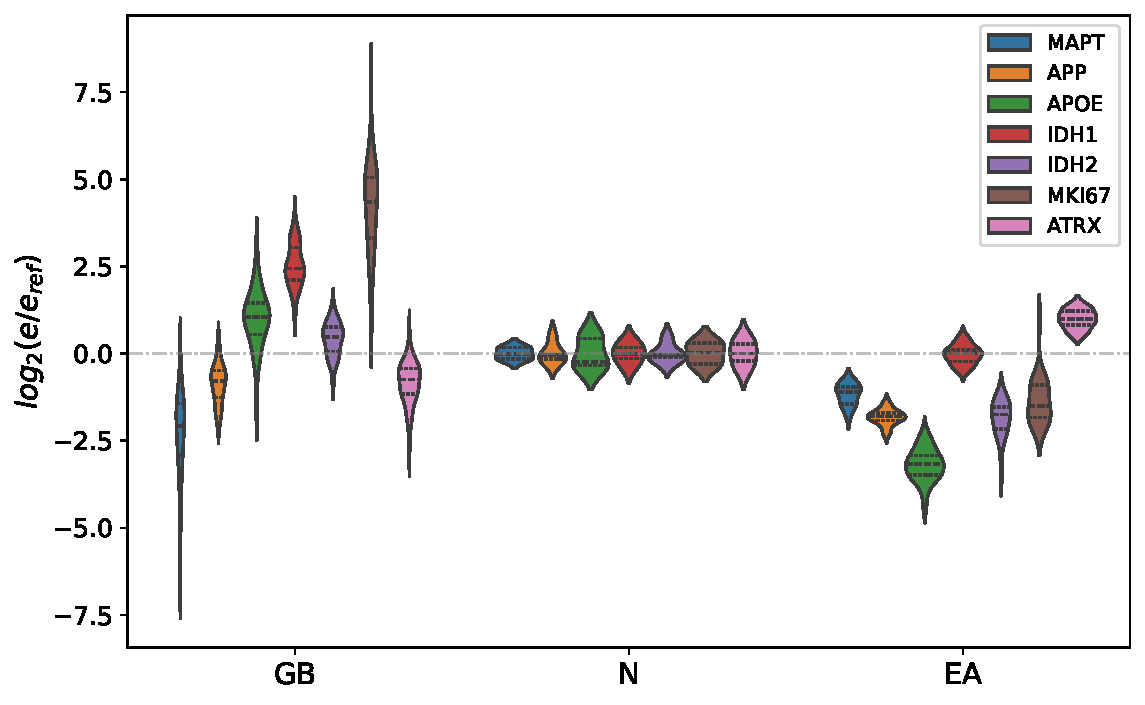
\includegraphics[width=\linewidth]{figures/suppl2}
	\caption{Gráficos de violín para marcadores conocidos en la EA y el GB.}
	\label{fig:violin}
\end{figure}

Por otro lado, el marcador IDH1 \cite{Cohen_2013} está sobreexpresado en la GB, pero es irrelevante en la EA. Los tres marcadores de GB, IDH2 \cite{Cohen_2013}, MKI67 \cite{Chen_2015} y ATRX \cite{Haase_2018}, son genes similares a PC2. Se han estudiado principalmente en relación con la GB, pero el hecho de que sean genes PC2 indica que podrían desempeñar un papel importante también en la EA.

Consideremos, como último ejemplo, la reciente demostración de la relevancia de TREM2 en la EA \cite{van_Lengerich_2023}. Se ha demostrado que la activación de TREM2 en la EA mejora el metabolismo microglial. Según nuestro análisis, TREM2 es un gen PC2, subexpresado en la EA y sobreexpresado en el GB. Por lo tanto, esperamos que la inhibición de TREM2 en células de glioblastoma pueda tener un efecto importante en el GB. Este hecho, según nuestro sencillo esquema, se encuentra actualmente en estudio \cite{Sun_2023}.


%    \input{./cap4}
    % !TeX root = Tesis.tex
% !TeX encoding = UTF-8
% !TeX spellcheck = es_ES
\chapter*{Conclusiones}\label{conclutions}
\addcontentsline{toc}{chapter}{Conclusiones}
\onehalfspacing

Nuestros sencillos esquemas cualitativos identifican direcciones en el espacio de expresión genética asociadas a diferentes procesos biológicos: envejecimiento, carcinogénesis, aparición de la enfermedad de Alzheimer. Cada una de estas direcciones se caracteriza por un "metagén" o perfil de expresión genética, del cual se pueden extraer los principales genes que contribuyen al proceso.

Algunos de nuestros resultados confirman conocimientos previos, pero otros requieren mayor corroboración. Por ejemplo, la idea de que el envejecimiento programático podría estar relacionado con evitar el fuerte atractor GB, o la aparición tardía de la EA como la captura por el atractor de EA de muestras de edad normal. Esperamos que estos resultados motiven la investigación experimental en estas direcciones. El experimento en un modelo de ratones es particularmente factible, como lo demuestra la referencia \cite{hahn2023atlas}.

Cabe destacar que incluso datos o métodos computacionales más refinados no podrían modificar sustancialmente nuestros esquemas cualitativos con solo tres atractores. Sus posiciones relativas podrían variar, pero las afirmaciones formuladas se mantendrán.


\chapter*{Recomendaciones}\label{recomendations}
\addcontentsline{toc}{chapter}{Recomendaciones}

El diagrama de la Fig. \ref{fig:fig1a} debe completarse con datos correspondientes a otros tipos de demencia o trastornos cerebrales. En particular, se espera un área de la enfermedad de Parkinson cercana al atractor de la EA y opuesta al GB \cite{Mencke_2020}. El panorama completo puede revelar una topología aún más precisa del espacio de expresión genética y un diagrama de Wright más completo.

Anticipamos que diagramas similares en otros tejidos, además de proporcionar una perspectiva integral, podrían ser útiles en la comprensión de la biología de enfermedades o trastornos aparentemente no relacionados, y en el descubrimiento de pistas inesperadas para su tratamiento.


	
     %\input{./Pseudocodigo}
%     \input{./Ajuste}
     %Si hay más apéndices, solo los agregas
     


	\backmatter

	\singlespacing
	\bibliographystyle{ieeetr}  % or: plain,unsrt,alpha,abbrv,acm,apalike, ieeetr,..
%    \bibliographystyle{phd_bib}	% definir el estilo de la bibliografía .bst (phd_bib,mibib)
    \bibliography{bibl} 	% ejemplo. hacer uno genérico. Solo pone las que se citan.
%    \bibliography{test}
%    \nocite{*}

%	\singlespacing
%	\appendix
%%	\section*{Apéndices}
%	\addcontentsline{toc}{chapter}{Apéndices}
%	\input{./microarray-example}
%	\input{./tablas}

\end{document}
